\section{Introduction}
In this chapter, procedure and packages are discussed. Procedures are similar to functions in python, which is used to define common operations. Further, packages are used to define common declarations in one file, instead of declaring in each file as shown in Chapter \ref{ch:OverView}. 

\section{Procedure}
A procedure contains a list of input and outputs arguments, and defined in declaration part of the architecture as shown in lines 19-25 of Listing \ref{vhdl:procedureEx}. 

\begin{explanation}[Listing \ref{vhdl:procedureEx}]
	In line 19, `sum2Num' is the name of the procedure, which has two input signal (a and b) and two output signals (sum and diff). Then, line 27 maps the input and output port of the entity to this procedure. Note that signal `p' is mapped to `sum' signal, therefore line 28 is used to assign the value of `p' to output port `d'. Fig. \ref{fig:procedureEx} is the design generated by the listing, whereas  Fig. \ref{fig:procedureExWave} is the simulation waveforms. 
\end{explanation}
\lstinputlisting[
language = Vhdl,
caption    = {Procedure},
label      = {vhdl:procedureEx}
]{procedureEx.vhd}

\begin{figure}[!h]
	\centering
	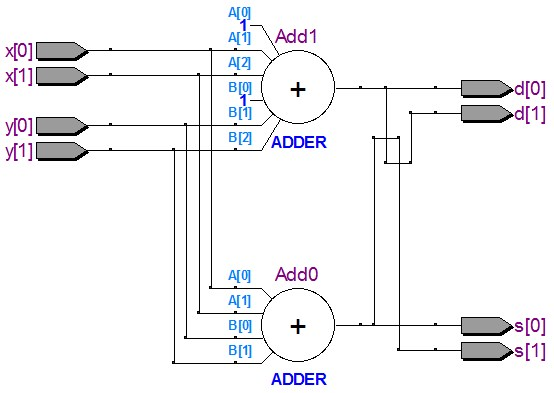
\includegraphics[scale=0.5]{procedureEx}
	\caption{Design generated by Listing \ref{vhdl:procedureEx}}
	\label{fig:procedureEx}
\end{figure}

\begin{figure}[!h]
	\centering
	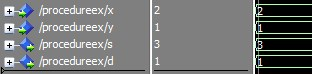
\includegraphics[scale = 1.2]{procedureExWave}
	\caption{Waveform for Listing \ref{vhdl:procedureEx}}
	\label{fig:procedureExWave}
\end{figure}

\section{Packages}
Packages are already discussed in Chapter \ref{ch:OverView}. In this section, package body is discussed using Listing \ref{vhdl:myPackage} and \ref{vhdl:packageCall}.

\begin{explanation}[Listing \ref{vhdl:myPackage}]
	In the listing constants (line 9), signals (line 17), data-types (line 18) and procedure (line 12) are defined inside the package `myPackage'. Further, procedure is declared in the package (line 12-19), and then defined in the package body (line 24-29). All these declarations are used by Listing \ref{vhdl:packageCall}. 
\end{explanation}

\lstinputlisting[
language = Vhdl,
caption    = {Package},
label      = {vhdl:myPackage}
]{myPackage.vhd}

\begin{explanation}[Listing \ref{vhdl:packageCall}]
	In this listing, line 6 adds all the declaration of `myPackage' to current design. Note that, `work' is the default directory where all the compiled file are stored. 
	\\ \\
	Next, line 30 adds two number, in which `S' is defined in the package. 
	\\ \\
	Line 33 is using the procedure `sum2Num' which is declared in the package. The working of this part is same as Listing \ref{vhdl:procedureEx}. 
	\\ \\
	Line 26 defines the signal `currentState' of type `stateType' which is declared in package. Similarly, signal `f' used in line 38 which is also defined in the package. Rest of the working of line 38-55 is same as Listing \ref{vhdl:ifLoop}.
\end{explanation}

\lstinputlisting[
language = Vhdl,
caption    = {Adding Package to current design},
label      = {vhdl:packageCall}
]{packageCall.vhd}

\section{Conclusion}
In this chapter, we discuss the procedure and package. We define some of the previous designs in the package, and then use the package to create new design. 